% !TeX root = ../HebutThesis_example.tex(此文件是被HebutThesis_example.tex调用的)
\chapter{绪论}
\setcounter{page}{1}
\pagenumbering{arabic}



\section{研究背景与意义}
%人工智能影响生活
%生成算法在人工智能领域的地位
%中国画当前情况
%中国画生成算法研究的意义
在当今时代,人工智能技术与我们日常生活的联系逐渐紧密。
智能手机、智能家居等智能设施让我们的生活更加便利,影视作品、新闻报道中也常常出现与人工智能有关内容。
理查德·费曼曾经说过:“我无法创造我所不理解的事物”,对生成模型的研究有助于让人工智能更加“理解”现实世界。
中国画{\cite{chinesepainting}}是我国传统的绘画形式,其在内容和艺术创作上,体现了古人对自然、社会及与之相关联的政治、哲学、宗教、道德、文艺及自然等方面的认识。
使用生成模型算法进行中国画创作,有助于继承和弘扬我国优秀传统文化,让中国画在新时代焕发新的光彩。









\section{国内外研究现状}
%生成模型当前情况
%人工智能
%机器学习
%深度学习
%生成模型
%生成模型算法在中国画生成方面研究
1950年,艾伦·图灵提出著名的“图灵测试” {\cite{machinery1950computing}},给出了判定机器是否具有“智能”的试验方法,即机器是否能够模仿人类的思维方式来“生成”内容继而与人交互。
某种程度上来说,人工智能从那时起就被给寄予了用于内容创造的期许{\cite{aigcwhitebook}}。
最初,人们尝试通过编码,将具体的规则赋予人工智能,但面临的各种困难使人们转变策略。
不再是直接提供人为设定的规则,而是为人工智能提供数据资料,让人工智能从数据资料中“学习”所需的规则,也就是“机器学习” {\cite{goodfellow2016deep}}。
随着计算机运算能力的增加与数据量的增长,在机器学习中,让计算模型通过多个中间层来逐渐理解数据潜在表示的“深度学习” {\cite{lecun2015deep}},逐渐在计算机视觉、自然语言处理、语音识别等领域取得了突破。

深度学习与生成模型的结合,让人工智能生成内容迎来了新时代,生成内容百花齐放,效果逐渐逼真直至人类难以分辨。

\subsection{2014--2017 变分自编码器和生成对抗网络时代}
2013年,变分自编码器 {\cite{kingma2013auto}}的提出使人们认识到,生成模型不仅可以生成简单的数字图像,还可以生成像人脸一样更复杂的图像。生成的图像可以随着隐空间取值的变化而变化。
2014年,生成对抗模型 {\cite{goodfellow2020generative}}的提出,为人们提供了一种通过对抗结构来解决生成模型问题的全新思路。
在随后三年内,人们对生成对抗网络进行了扩展与改进,
如对基础模型结构进行改进的DCGAN {\cite{radford2015unsupervised}},
对损失函数进行改进的Wassertein GAN {\cite{arjovsky2017wasserstein}},
对训练过程进行改进的ProGAN {\cite{karras2017progressive}},
还有使用生成对抗网络在新的领域进行应用,如图像与图像的转化 {\cite{isola2017image}\cite{zhu2017unpaired}}以及音乐的生成 {\cite{dong2018musegan}}。

在同时期,变分自编码器也有了一些重要的改进,如VAE-GAN {\cite{larsen2016autoencoding}}和随后的VQ-VAE {\cite{razavi2019generating}},以及在强化学习上的应用 {\cite{ha2018world}}。

在文本生成领域,自回归模型如LSTMs和GRUs仍然是主流研究方向,相同的自回归思路也应用在图像生成领域,如PixelRNN {\cite{van2016pixel}}和PixelCNN {\cite{van2016conditional}}引入了一种新的生成图像的方式。
也有一些其他生成图像方式的尝试如RealNVP {\cite{dinh2016density}}的出现,为之后规范化流模型打下了基础。

2017年,Transformer {\cite{vaswani2017attention}}的提出使生成模型的研究转向Transformers。
\subsection{2018--2019 Transformer时代}
注意力机制是Transformer模型的核心,其使自回归模型不再需要循环层。随着只有Transformer解码器的GPT {\cite{radford2018improving}}以及只有Transformer编码器的BERT {\cite{devlin2018bert}}的提出,Transformer很快成为了研究的主流方向。
之后,越来越大的模型在很多生成文本的任务上取得了很好的效果。此外,Transformer也在音乐生成上取得了不错的效果 {\cite{huang2018music}}。

在这两年,一些重要的生成对抗网络模型的提出也巩固了其在图像生成领域的地位。
如SAGAN {\cite{zhang2019self}}和BigGAN {\cite{brock2018large}}将注意力机制引入生成对抗模型,取得了很好的效果,
StyleGAN {\cite{karras2019style}}和随后的StyleGAN2 {\cite{karras2020analyzing}}向人们展示了如何控制生成图像的风格与内容。

另一方面,基于分数的模型NCSN {\cite{song2019generative}}的提出,为扩散模型的出现打下了基础。
\subsection{2020--2023 大模型时代}
在此时期,一些模型将以往不同种类的模型混合,并在此基础上进一步改进。
如VQ-GAN {\cite{esser2021taming}}将生成对抗网络的判别器引入VQ-VAE模型结构,Vision Transformer {\cite{dosovitskiy2020image}}将Transformer应用在图像领域。
2022年,StyleGAN-XL {\cite{sauer2022stylegan}}对StyleGAN的进一步改进,使其能够在更大的数据集上生成更高分辨率的图像。

于2020年提出的两个模型——DDPM {\cite{ho2020denoising}}和DDIM {\cite{song2020denoising}},为之后的大规模图像生成模型打下基础。
在图像生成领域,突然出现的扩散模型成为了生成对抗网络的竞争对手。
扩散模型不仅可以生成高质量图像,相比于生成对抗网络也更容易训练。

在2020年同一时期,拥有1750亿参数的GPT-3 {\cite{brown2020language}}发布,其可以生成关于任何主题的文本内容。
在2022年,OpenAI在GPT-3基础上发布网页应用ChatGPT,让用户可以与ChatGPT自然地交流。

在2021年到2022年,一些在大规模语料库上训练的Transformer的变体模型也涌现而出,如微软和英伟达发布的Megatron-Turing NLG {\cite{smith2022using}},谷歌发布的LaMDA {\cite{thoppilan2022lamda}}等。

在过去两年,由于Transformer系列模型在文本生成领域的成功,以及扩散模型在图像生成领域的应用,人们开始关注多模态内容生成的研究,如使用文本生成图像。
如OpenAI在2021年发布的模型DALL.E {\cite{ramesh2021zero}},随后的GLIDE {\cite{nichol2021glide}}和DALL.E 2 {\cite{ramesh2022hierarchical}},谷歌发布的Imagen {\cite{saharia2022photorealistic}}、Parti {\cite{yu2022scaling}}和MUSE以及Stability AI发布的Stable Diffusion {\cite{rombach2022high}}等。
\section{研究内容与创新点}
%对各类生成算法进行原理探究
%使用扩散模型生成中国画
生成模型算法近年来发展较为迅速,但仍缺少资料对生成模型进行较为系统的探索与研究。
如今主流生成模型有规范化流模型、自回归模型、基于能量的模型、变分自编码器、扩散模型和生成对抗网络,
各类模型最先进的算法都可以取得很好的效果,
但生成模型为什么这样设计,其真正原理是什么,各种生成模型之间有什么关系,
理解这些问题有助于设计更好的生成模型,以达到更好的生成效果。
本文为首次对各种生成模型原理进行介绍,并将各种框架纳入同一体系的,
以有助于研究人员对生成模型进一步研究。

此外,中国画为传统艺术形式,但近年来相比于西方绘画技术的普及,中国画逐渐式微。
本文对生成模型在中国画生成方面进行探索,以期望使用人工智能技术生成高质量中国画,继承与弘扬中华传统文化。





\section{论文组织结构}

第一章首先介绍研究背景与意义,
随后介绍早期人工智能生成模型情况,
再将近年来生成模型发展分为三个阶段,
2014–2017为变分自编码器和生成对抗网络时代,
2018–2019为Transformer时代
2020–2023为大模型时代。
随后介绍研究内容与创新点与论文组织结构。

第二章首先介绍生成模型算法基本理论与生成模型用途,
再根据如何表示或近似似然函数将生成模型分为三类,
分别为可求解的显示密度模型、
近似估计的显示密度模型和隐式密度模型。
其中可求解的显示密度模型与近似估计的显示密度模型都属于显式密度模型。
如图{\ref{fig:gennerative_models}}所示,
可求解密度模型包含规范化流模型和自回归模型,
近似估计密度模型包含基于能量的模型、变分自编码器和扩散模型。
{\ref{section:explicit_density_model}}对各显式密度模型进行了详细介绍,
{\ref{section:implicit_density_model}}对隐式密度模型生成对抗网络进行了详细介绍,
最后,介绍了生成模型评价方法。
\begin{figure}[ht]
    \centering
    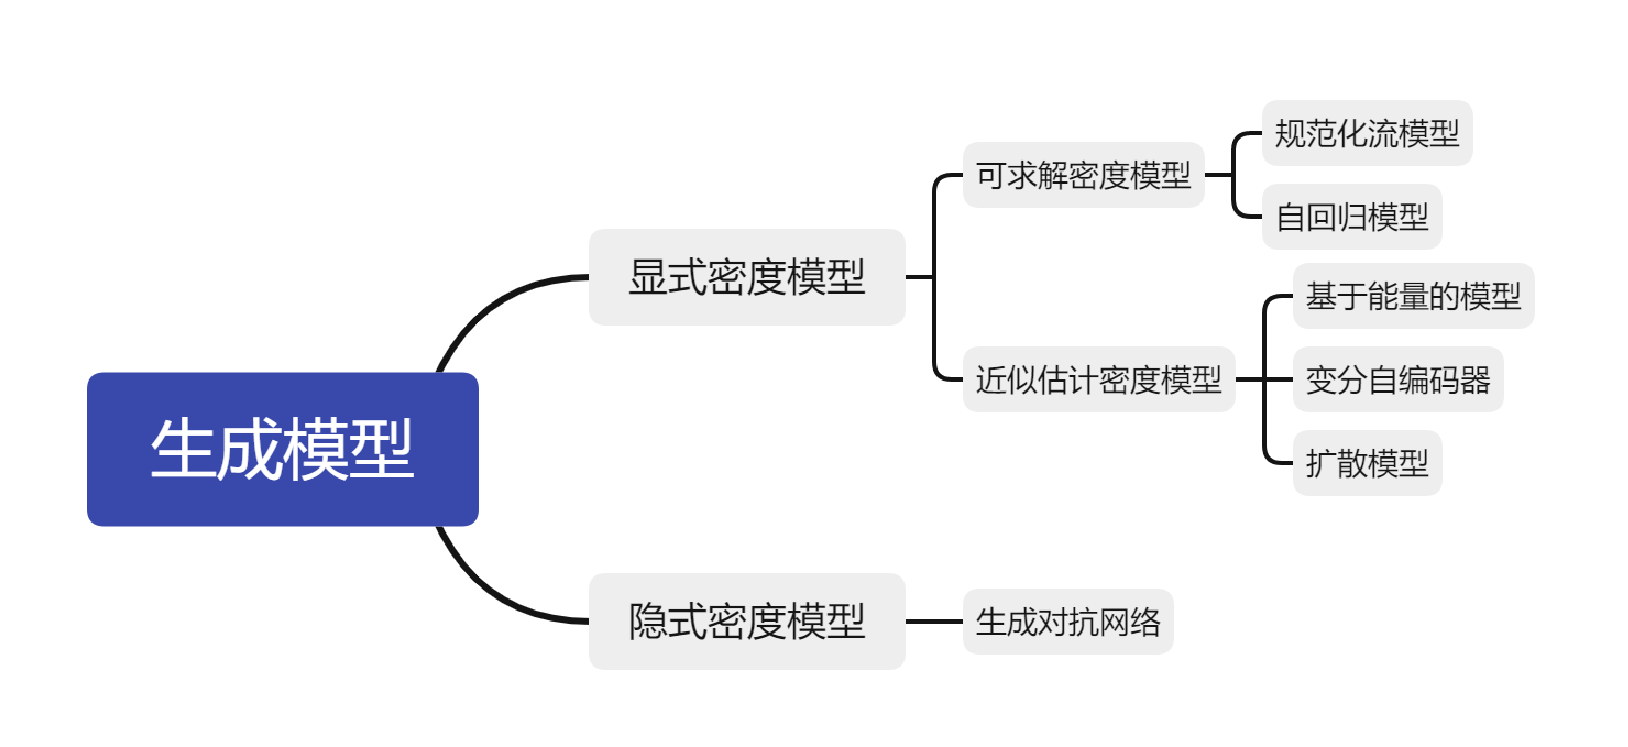
\includegraphics[width=\textwidth]{figures/gennerative_models}
    \caption{生成模型分类}\label{fig:gennerative_models}
\end{figure}



第三章使用扩散模型进行中国画生成,
根据所使用数据集与训练超参数不同,
生成不同类型的中国画。

最后对各生成模型算法与中国画生成进行总结与展望。

此外,为保持文中推理证明的完整性,在附录中添加证明所用基础知识。

% 第二章首先介绍生成模型算法基本理论,
% 第三章在变分自编码器模型基础上进行中国画生成,
% 第四章在自回归模型基础上进行中国画生成,
% 第五章在基于能量的模型基础上进行中国画生成,
% 第六章在规范化流模型基础上进行中国画生成,
% 第七章在生成对抗网络模型基础上进行中国画生成,
% 第八章在降噪扩散模型基础上进行中国画生成,
% 第九章对生成模型算法以及其在中国画上应用进行总结与展望。